\documentclass[
   a4paper,
   oneside,
   parskip=half,
   listof=entryprefix,
   listof=totoc,
   index=totoc,
   bibliography=totoc
]{scrartcl}

\usepackage{silence}
\WarningFilter{biblatex}{File 'ngerman-iso.lbx'}
\WarningFilter{biblatex}{'\mainlang'}

\usepackage[utf8]{inputenc}
\usepackage[ngerman]{babel}
\usepackage[T1]{fontenc}

\usepackage{pdfpages,graphicx,subcaption,lastpage}
\graphicspath{ {./images} }

\usepackage{geometry}
\geometry{a4paper, top=2.5cm, left=2.5cm, right=2.5cm, bottom=2.5cm}
\usepackage{float,listings,xcolor,csquotes,microtype,scrlayer-scrpage,etoolbox}
\usepackage[official]{eurosym}

\definecolor{codegreen}{rgb}{0,0.6,0}
\definecolor{codegray}{rgb}{0.5,0.5,0.5}
\definecolor{codepurple}{rgb}{0.58,0,0.82}
\definecolor{backcolour}{rgb}{0.95,0.95,0.92}
\definecolor{weborange}{rgb}{1,0.65,0}

\lstdefinestyle{mystyle}{
    backgroundcolor=\color{backcolour},   
    commentstyle=\color{codegreen},
    keywordstyle=\color{magenta},
    numberstyle=\tiny\color{codegray},
    stringstyle=\color{codepurple},
    emph={int,char,double,float,unsigned,void,bool},
    emphstyle={\color{weborange}},
    basicstyle=\ttfamily\footnotesize,
    breakatwhitespace=false,
    breaklines=true,
    captionpos=b,
    keepspaces=true,
    numbers=left,
    numbersep=5pt,
    showspaces=false,
    showstringspaces=false,
    showtabs=false,
    tabsize=2,
    firstnumber=1,
}
\lstset{style=mystyle}

\setuptoc{toc}{totoc}

\usepackage[
   backend=biber,
   urldate=long,
   style=iso-authoryear,
   natbib=true,
   useauthor=true,
   mincitenames=1,
   maxcitenames=3
]{biblatex}
\addbibresource{bib/online.bib}
\addbibresource{bib/book.bib}

\DefineBibliographyStrings{ngerman}{
   andothers = {{et\,al\adddot}},
   online = {{online}},
   urlseen = {{Zugriff am:}},
   urlfrom = {{Verfügbar unter:}},
}

\DeclareNameAlias{default}{family-given/given-family}

\renewcommand*{\finalnamedelim}{\addspace{}und\space}
\AtEveryCite{
   \renewcommand*{\multinamedelim}{,\space}
   \renewcommand*{\nameyeardelim}{\space}
}

\AtBeginBibliography{
   \renewcommand*{\multinamedelim}{,\space}
}
\AfterTOCHead[lof]{\appto\autodot{:}}

\definecolor{must-have-brown}{RGB}{51, 22, 18}
\definecolor{should-have-red}{RGB}{229, 24, 31}
\definecolor{could-have-orange}{RGB}{246, 121, 28}
\definecolor{wont-have-blue}{RGB}{32, 169, 215}
\newcommand{\morequirement}[1]{\paragraph{#1}\hfill\textbf{\textcolor{must-have-brown}{must-have}}\\}
\newcommand{\srequirement}[1]{\paragraph{#1}\hfill\textbf{\textcolor{should-have-red}{should-have}}\\}
\newcommand{\corequirement}[1]{\paragraph{#1}\hfill\textbf{\textcolor{could-have-orange}{could-have}}\\}
\newcommand{\wrequirement}[1]{\paragraph{#1}\hfill\textbf{\textcolor{wont-have-blue}{won't-have}}\\}

\ihead{Example Header}
\chead{}
\ohead{Surname Lastname}
\ofoot{Seite~\thepage{}/\pageref{LastPage}}
\cfoot{}
\title{Example Title}
\usepackage[breaklinks,colorlinks,linkcolor=black,citecolor=black,filecolor=black,urlcolor=black]{hyperref}

\begin{document}

    \newcommand{\HRule}[2]{\noindent\rule[#1]{\linewidth}{#2}}
\newcommand{\vlinespace}[1]{\vspace*{#1\baselineskip}}
\newcommand{\titleemph}[1]{\textbf{#1}}
\begin{titlepage}
    \sffamily
    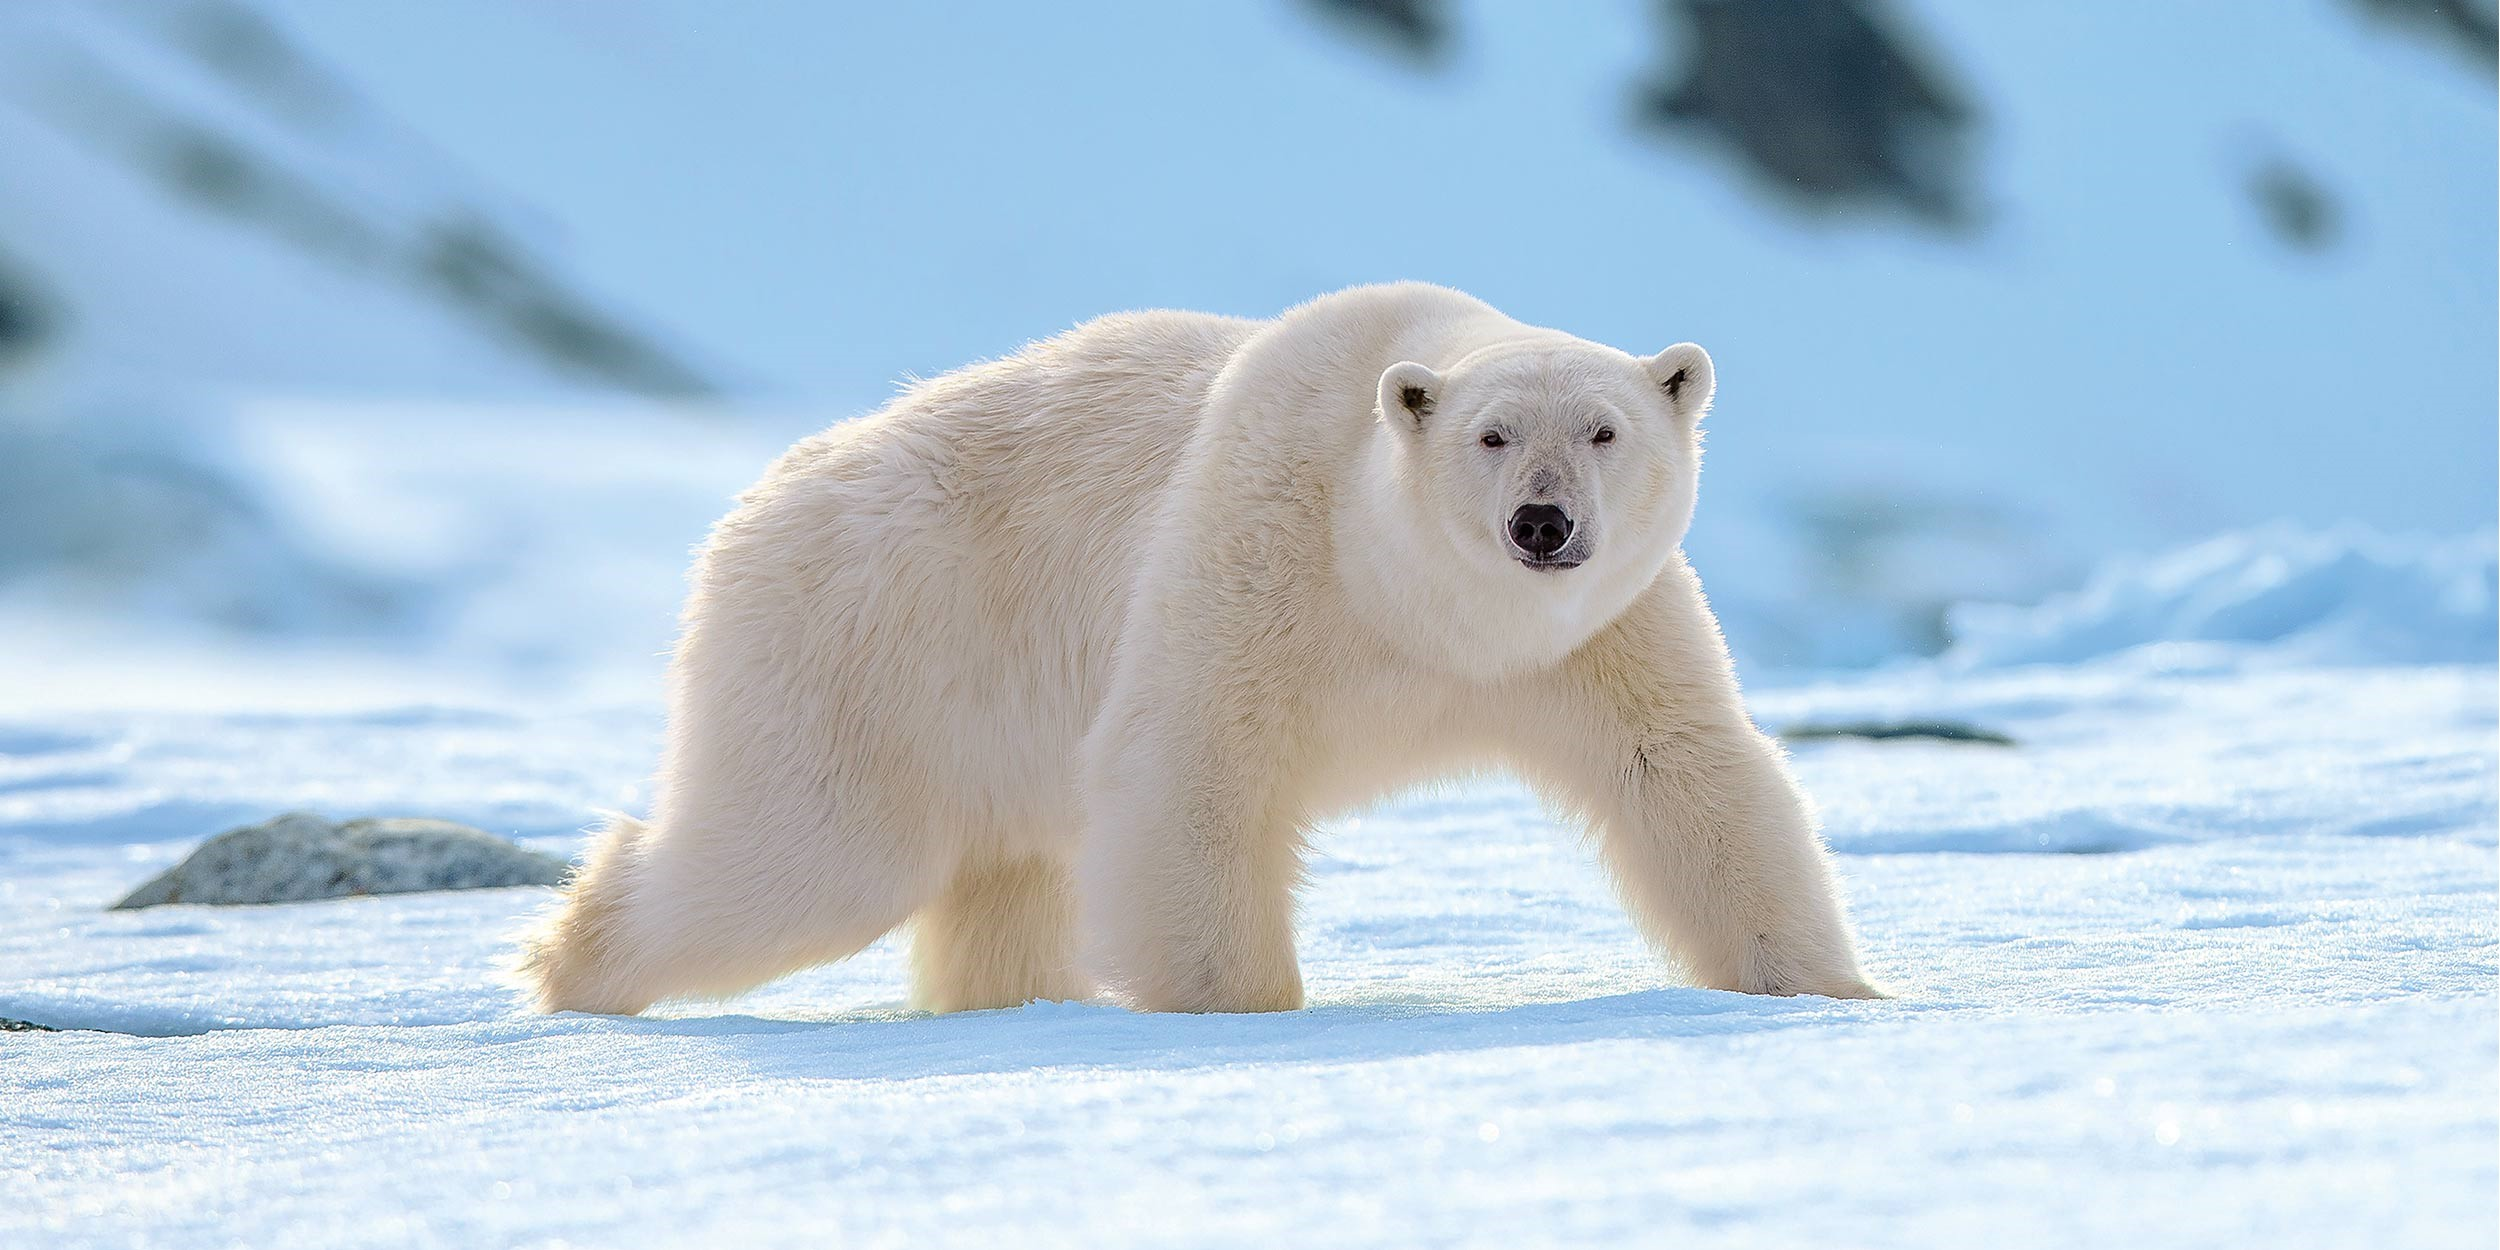
\includegraphics[width=5cm]{example}
    \hfill
    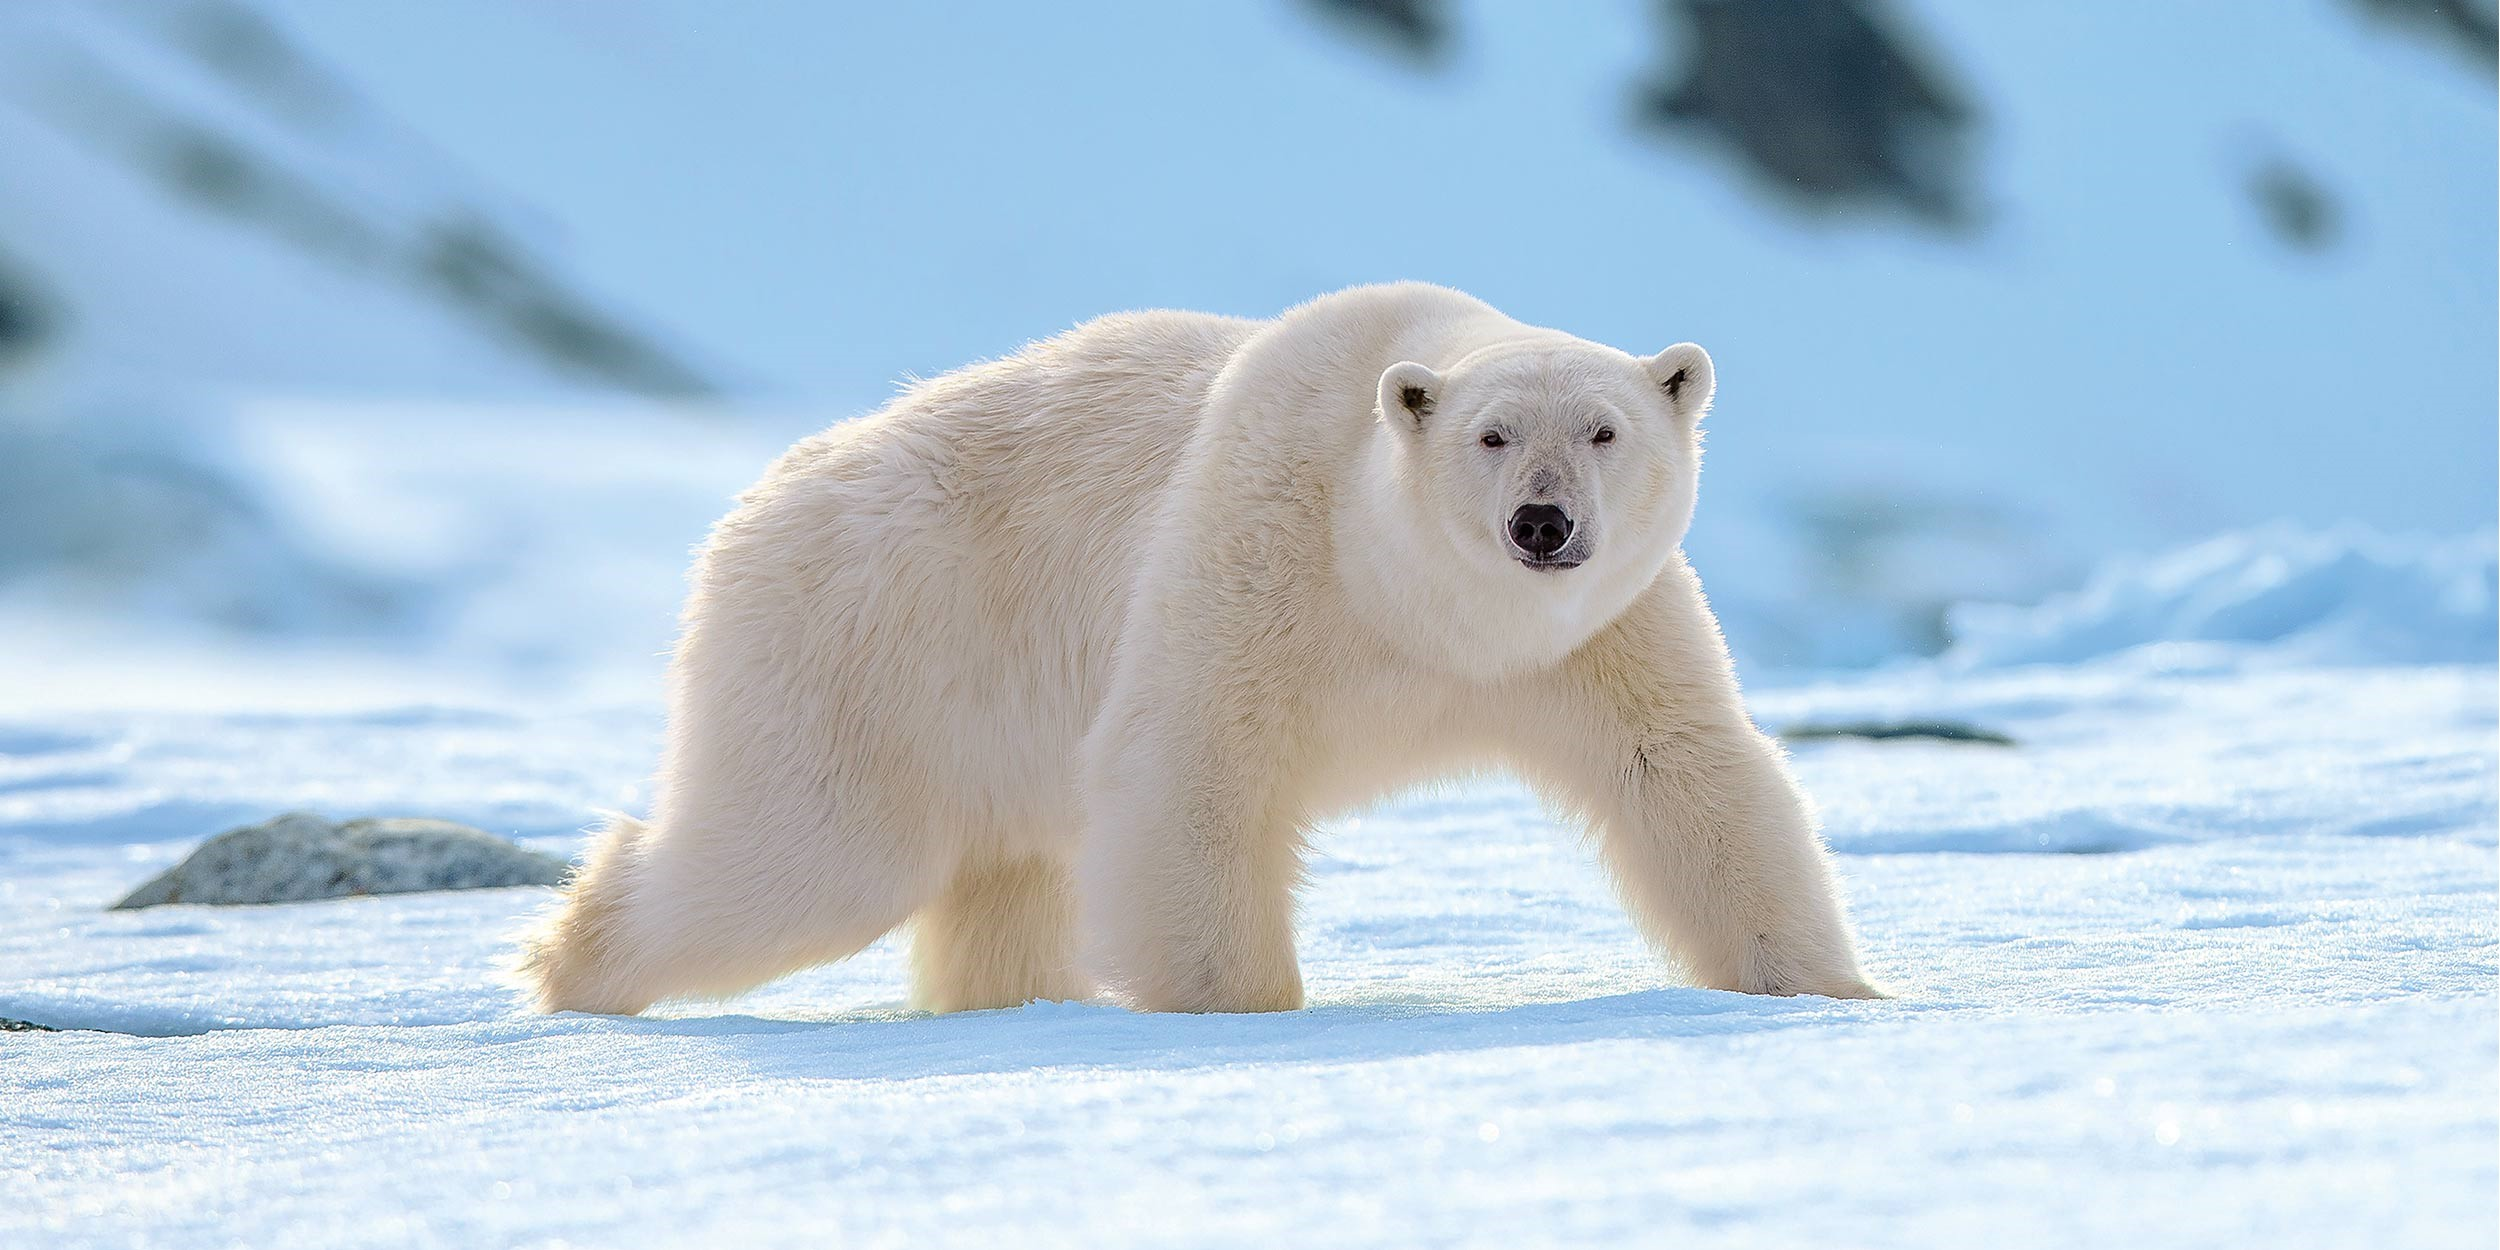
\includegraphics[width=5cm]{example}
    \HRule{13pt}{1pt}
    \centering
    \vlinespace{5}\\
    \workTyp\\
    \begin{Large}
        \textbf{Titel}\\
        \textbf{und mehr}\\
    \end{Large}
    \vlinespace{4}
    im Studiengang\\
    <Studiengang>\\
    am \workDatum\\
    \vlinespace{4}
    vorgelegt von\\
    \begin{Large}
        \textbf{\workNameStudent}\\
    \end{Large}
    \vlinespace{1}
    Matrikelnummer: <12345>
    \vfill
    \raggedright{}
    \HRule{13pt}{1pt} \\
    \titleemph{Erstprüfer:} Prof. <wx>\\
    \titleemph{Zweitprüfer:} Prof. <yz>
\end{titlepage}
    \tableofcontents
    \newpage
    \listoffigures
    \section{Example}

\begin{figure}[H]
    \begin{center} 
        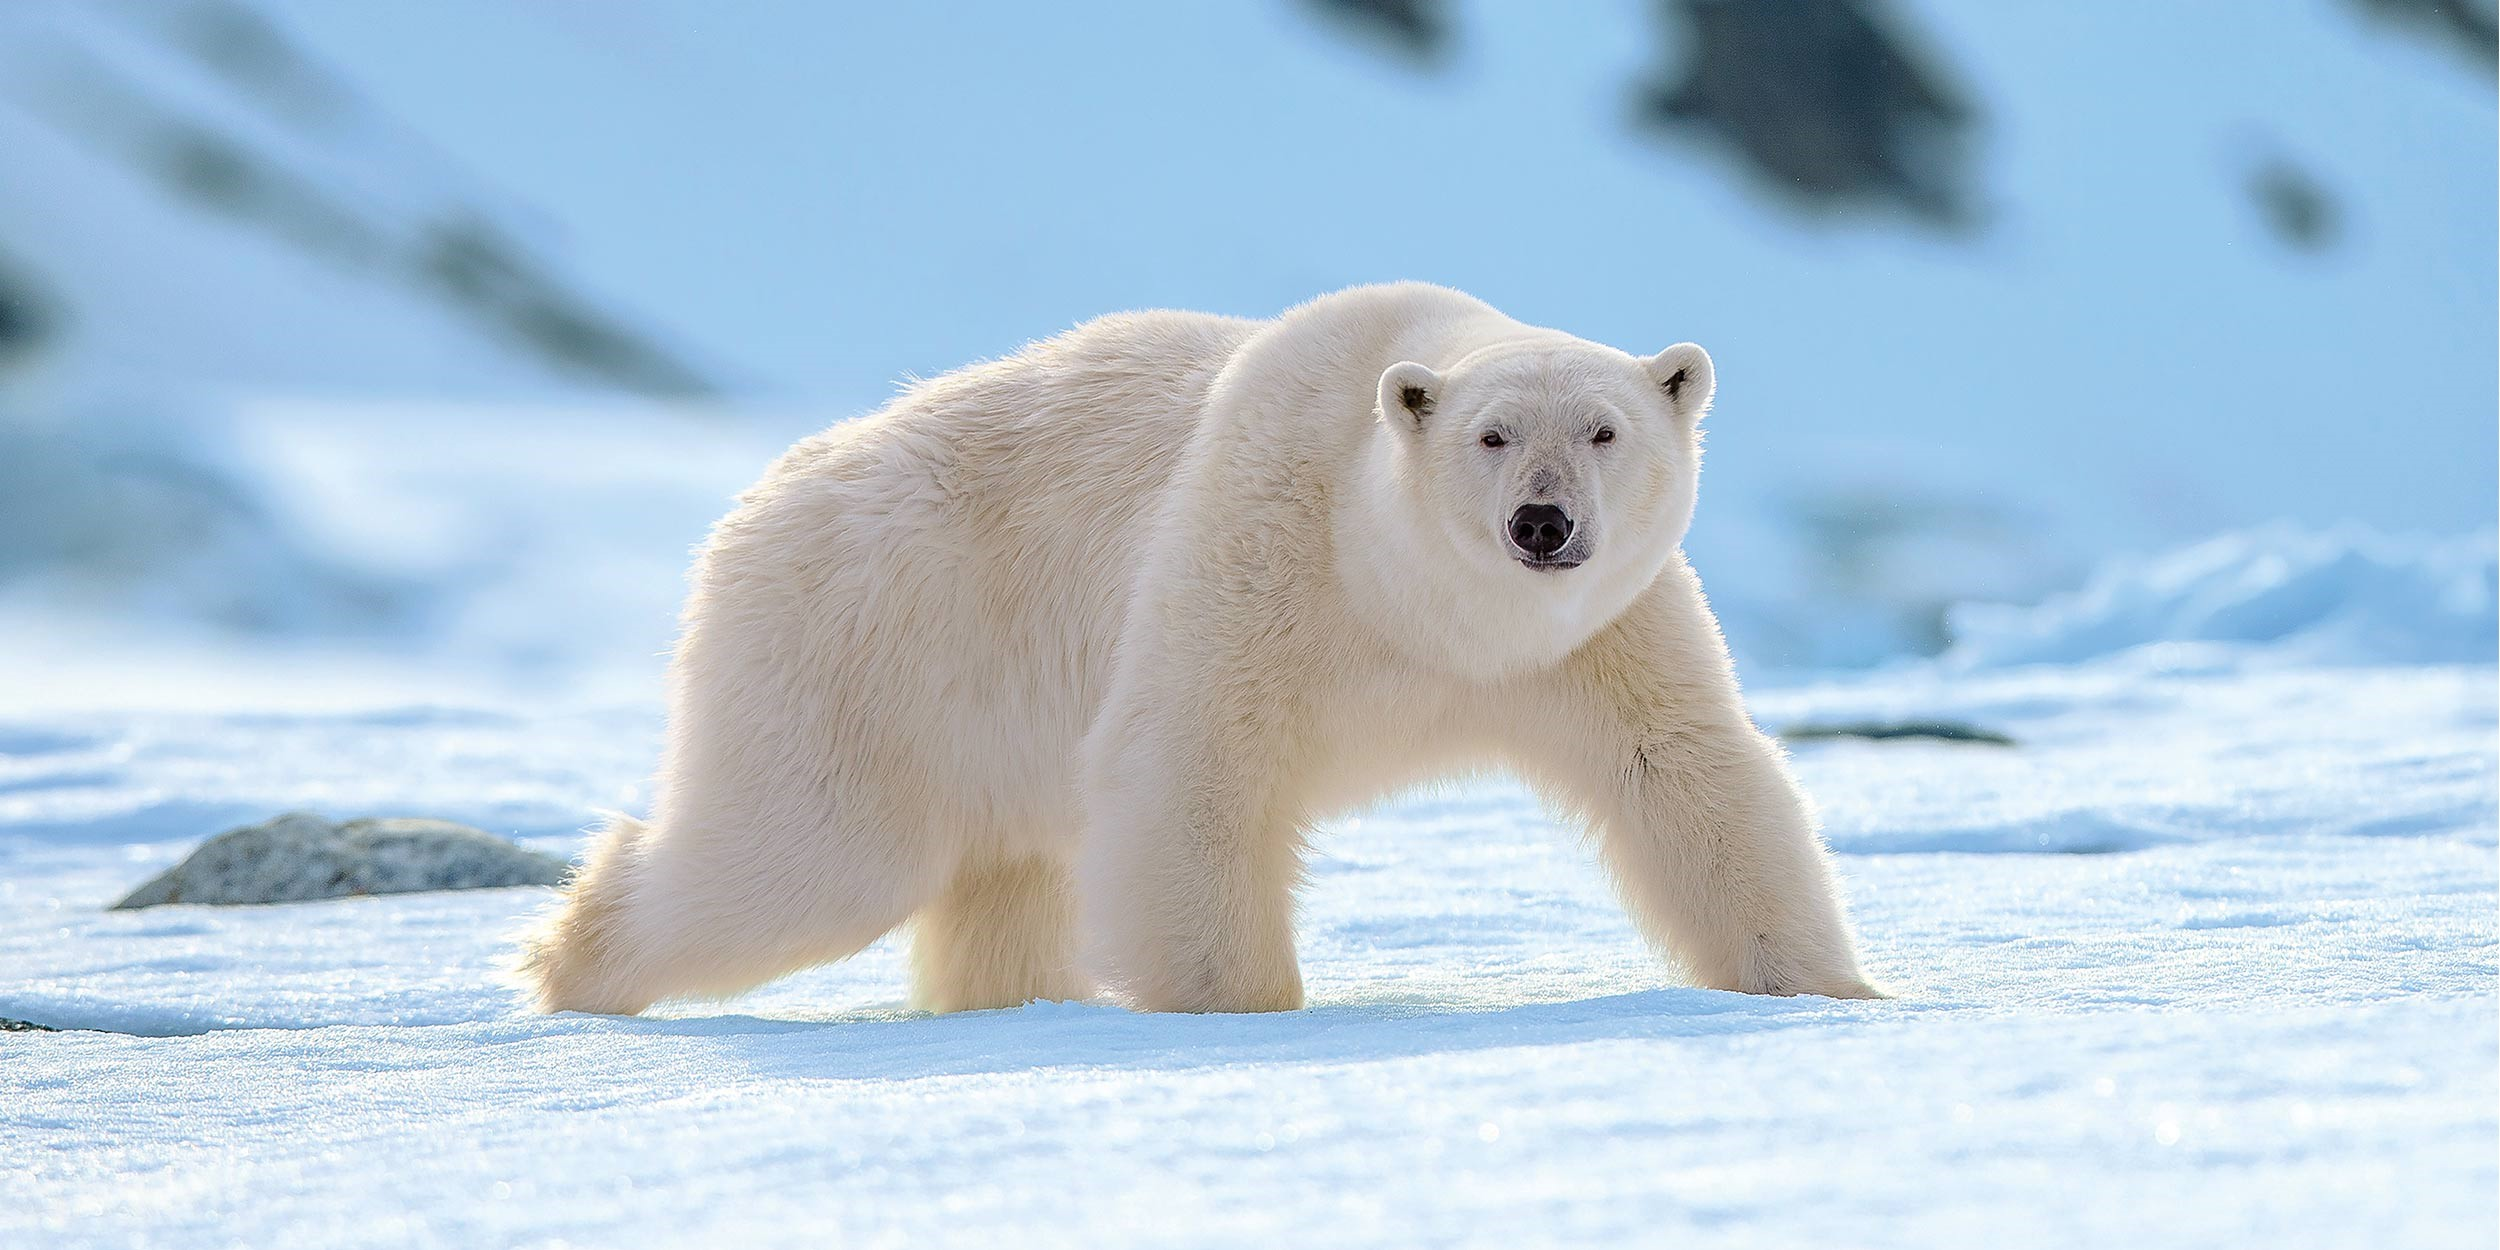
\includegraphics[width=0.8\textwidth]{example}
        \caption{Example Image}
        \label{fig:example}
    \end{center}
\end{figure}

\cite[vgl. dazu][]{example-book}

\cite[vgl. dazu][]{example-online}

\newpage

\begin{lstlisting}[language=Bash]
#!/bin/bash

echo "Hello World"
\end{lstlisting}

\begin{lstlisting}[language=Python]
# same in python

print("Hello World")
\end{lstlisting}

\begin{verbatim}
$ sudo apt-get update
$ sudo apt-get install python
\end{verbatim}


    \printbibliography[title=Literaturverzeichnis]

\end{document}